\chapter{音声認識精度と検索精度}

% 全体の流れ
% NTCIR12で, CSJを用いたKALDIの認識結果が得られた.

2014年12月に開催されたNTCIR11では,音声認識結果の文書にJuliusによる認識結果が公開された.NTCIR12では,その認識結果の文書に加え,Kaldiを用いた認識結果の文書が公開された.Kaldiは,Kaldiはディープニューラルネットワーク(DNN)ベースの大語彙音声認識を行っており,高性能な認識システムの構築がされており,認識精度が高い.本章では,二つの認識エンジンを利用し,検索精度の違いが,認識結果に与える影響と分析する.

% juliusとか
% http://www.ar.media.kyoto-u.ac.jp/lab/bib/jpn/KAW-orc04.pdf
% http://www.cl.ics.tut.ac.jp/~sdpwg/sdpws2010_proceedings/SDPWS2010-16_shichiri.pdf
% wer 30%ぐらい

% 参考: http://www.ar.media.kyoto-u.ac.jp/lab/project/paper/RI-HIS09.pdf
\section{Julius}
Juliusは大語彙連続音声認識を実行するソフトウェアである.これまでの音声認識の研究で培われてきたアルゴリズムや計算効率化手法をおよそ実装しており,高精度かつ効率よく認識処理を行うことができる.
juliusの最も大きな特徴は汎用性・可搬性にある.音響モデルや言語モデルの仕様は標準的なフォーマットを採用しており,置き換えたり修正したりすることが容易である.これにより,大語彙のディクテーションから小語彙の数字認識まで,様々な使用環境や目的に応じたシステムを構築することが簡単にできる.また言語モデルも,大規模な統計モデルである単語n-gram,文パターンを人手で与える記述文法,辞書のみを用いる単語認識といったように多様な形式をサポートしており,使用環境に応じて適切なモデルを使い分けることができる.さらに,ソースコードが公開されているので,ユーザ独自の修正や拡張も可能である.

% TODO: 始めにいがいのネーミング
% 音響学会の論文参考
\section{Kaldi}
Kaldiはディープニューラルネットワーク(DNN)ベースの大語彙音声認識に対応した音声認識ツールキットであり,現在主に欧米において精力的に開発が進められ,音声認識研究において世界中に普及しつつある[1]Kaldiはオープンソースの音声認識ツールキットであり,C++で書かれたKaldi独自のコマンドプログラム, OpenFst等の既存ツールの自動インストーラ,各種コーパスを用いて音声認識システムの構築および認識実験を行うレシピなどにより構成されている.最新の認識技術が多く取り込まれており,高性能な認識システムの構築が可能となっている.
Kaldiでは音声認識研究で用いられる主要なコーパスに対して,学習データから音声認識システムを構築し認識性能を評価するまでの全プロセスを自動化したスクリプトが用意されている.これらのスクリプトは,レシピと呼ばれている.このレシピの中に、学習・評価データとして,日本語 話し言葉コーパス(CSJ) [2] に対応した,日本語のための音声認識レシピが公開されている.このレシピは,CSJ の標準評価セットを用いた認識実験において,全評価セットの平均で90.6\%と高い認識精度を実現している. NTCIR12では、このレシピを利用し,音声認識した結果の文書を提供している.


\section{評価実験}
\subsection{実験条件}
% NTCIR12の実験の詳細をどこかに掲載する

Juliusの音声認識結果とkaldiの音声認識結果の精度
の違いにおけるMAP値の変化を調べるために,実験を行う.実験でははまず,NTCIR12のformal-runクエリに対して,JuliusとKaldiでそれぞれ認識された検索対象文書とクエリを比較,コンテンツとしてマッチする文書をシステムが抽出する.また,書き起こしの検索文書よるMAP値も,比較のため提示する.

クエリの音声認識結果はJuliusの認識結果を利用する.文書の特徴量としてはクエリ尤度モデルにディリクレスムージングを施したものを利用し,そのときのMAP値を両者で比較する.

\subsection{実験結果}

表1より,MAP値はJuliusの音声認識文書,Kaldiの音声認識文書,書き起こし文書の順でMAP値が上昇していることが分かり,Juliusより生成された文書を利用するよりも,Kaldiを用いた文書を利用したほうが,MAP値がよいことが確認できた.

\begin{table}
    \centering
    \caption{書き起こし文書と認識文書を用いたときのMAP値}
    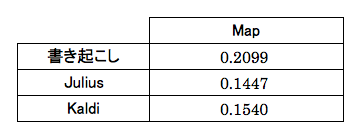
\includegraphics[width=7cm]{./image/write_julius_kaldi.png}
    \label{query_set}
\end{table}

% TODO: +α それぞれのAP値の比較・juliusとkalidがn/37の確率でどっちが上位か?